% Pares de transformadas de Fourier cl\'asicas
\documentclass[tikz,border=10pt]{standalone}
\usepackage{tikz}
\usepackage{amsmath}
\usetikzlibrary{arrows.meta, positioning, calc}

\definecolor{gdlblue}{RGB}{41, 98, 168}
\definecolor{gdlred}{RGB}{191, 49, 49}
\definecolor{gdlgreen}{RGB}{30, 130, 76}
\definecolor{gdlorange}{RGB}{217, 130, 30}
\definecolor{gdlpurple}{RGB}{118, 56, 138}
\definecolor{gdlgray}{RGB}{140, 140, 140}
\definecolor{gdlyellow}{RGB}{190, 140, 10}

\begin{document}
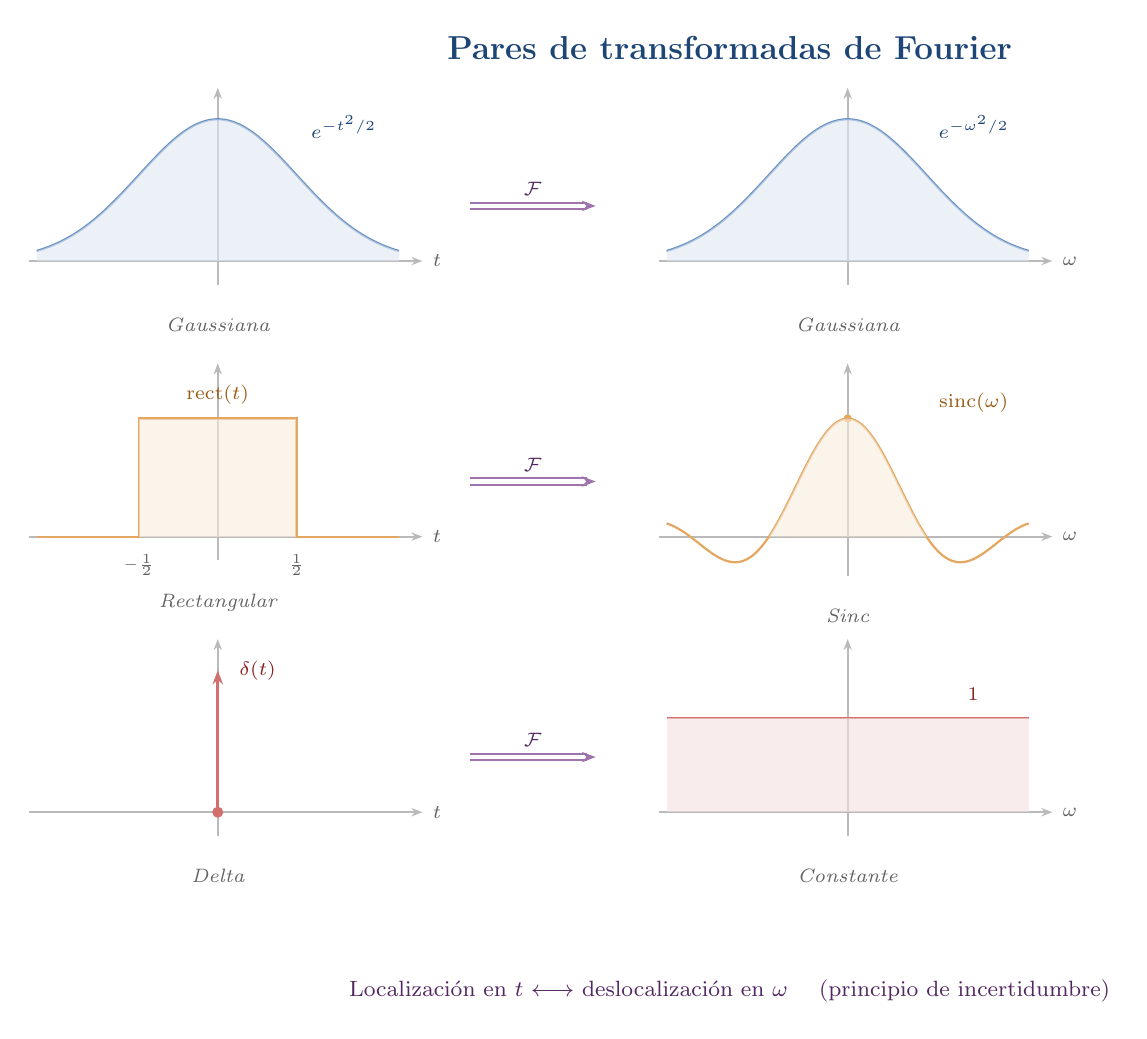
\begin{tikzpicture}

% === Title ===
\node[font=\bfseries\large, text=gdlblue!70!black] at (6.5, 1.2)
  {Pares de transformadas de Fourier};

% =====================================================================
% Row 1: Gaussian <-> Gaussian
% =====================================================================

% --- Time domain: Gaussian ---
\begin{scope}[shift={(0, -1.5)}]
  % Axes
  \draw[-{Stealth[length=4pt]}, gdlgray!60, thick] (-2.4, 0) -- (2.6, 0)
    node[right, font=\scriptsize, text=gdlgray!70!black] {$t$};
  \draw[-{Stealth[length=4pt]}, gdlgray!60, thick] (0, -0.3) -- (0, 2.2);
  % Gaussian curve: e^{-t^2/2}
  \draw[gdlblue!70, thick] plot[smooth, domain=-2.3:2.3, samples=60]
    (\x, {1.8*exp(-\x*\x/2)});
  % Fill
  \fill[gdlblue!15, opacity=0.6] plot[smooth, domain=-2.3:2.3, samples=60]
    (\x, {1.8*exp(-\x*\x/2)}) -- (2.3, 0) -- (-2.3, 0) -- cycle;
  % Label
  \node[font=\scriptsize, text=gdlblue!70!black] at (1.6, 1.7) {$e^{-t^2/2}$};
  % Subtitle
  \node[font=\scriptsize\itshape, text=gdlgray!70!black, anchor=north] at (0, -0.6)
    {Gaussiana};
\end{scope}

% --- Arrow ---
\draw[-{Stealth[length=5pt]}, gdlpurple!70, thick, double, double distance=1.5pt]
  (3.2, -0.8) -- (4.8, -0.8)
  node[midway, above, font=\scriptsize, text=gdlpurple!70!black] {$\mathcal{F}$};

% --- Frequency domain: Gaussian ---
\begin{scope}[shift={(8, -1.5)}]
  % Axes
  \draw[-{Stealth[length=4pt]}, gdlgray!60, thick] (-2.4, 0) -- (2.6, 0)
    node[right, font=\scriptsize, text=gdlgray!70!black] {$\omega$};
  \draw[-{Stealth[length=4pt]}, gdlgray!60, thick] (0, -0.3) -- (0, 2.2);
  % Gaussian curve: e^{-omega^2/2}
  \draw[gdlblue!70, thick] plot[smooth, domain=-2.3:2.3, samples=60]
    (\x, {1.8*exp(-\x*\x/2)});
  % Fill
  \fill[gdlblue!15, opacity=0.6] plot[smooth, domain=-2.3:2.3, samples=60]
    (\x, {1.8*exp(-\x*\x/2)}) -- (2.3, 0) -- (-2.3, 0) -- cycle;
  % Label
  \node[font=\scriptsize, text=gdlblue!70!black] at (1.6, 1.7) {$e^{-\omega^2/2}$};
  % Subtitle
  \node[font=\scriptsize\itshape, text=gdlgray!70!black, anchor=north] at (0, -0.6)
    {Gaussiana};
\end{scope}

% =====================================================================
% Row 2: Rectangular <-> Sinc
% =====================================================================

% --- Time domain: Box/rect function ---
\begin{scope}[shift={(0, -5.0)}]
  % Axes
  \draw[-{Stealth[length=4pt]}, gdlgray!60, thick] (-2.4, 0) -- (2.6, 0)
    node[right, font=\scriptsize, text=gdlgray!70!black] {$t$};
  \draw[-{Stealth[length=4pt]}, gdlgray!60, thick] (0, -0.3) -- (0, 2.2);
  % Box function
  \draw[gdlorange!70, thick]
    (-2.3, 0) -- (-1.0, 0) -- (-1.0, 1.5) -- (1.0, 1.5) -- (1.0, 0) -- (2.3, 0);
  % Fill
  \fill[gdlorange!15, opacity=0.6]
    (-1.0, 0) rectangle (1.0, 1.5);
  % Labels
  \node[font=\scriptsize, text=gdlorange!70!black] at (0, 1.8) {$\operatorname{rect}(t)$};
  \node[font=\tiny, text=gdlgray!70!black, anchor=north] at (-1.0, -0.1) {$-\frac{1}{2}$};
  \node[font=\tiny, text=gdlgray!70!black, anchor=north] at (1.0, -0.1) {$\frac{1}{2}$};
  % Subtitle
  \node[font=\scriptsize\itshape, text=gdlgray!70!black, anchor=north] at (0, -0.6)
    {Rectangular};
\end{scope}

% --- Arrow ---
\draw[-{Stealth[length=5pt]}, gdlpurple!70, thick, double, double distance=1.5pt]
  (3.2, -4.3) -- (4.8, -4.3)
  node[midway, above, font=\scriptsize, text=gdlpurple!70!black] {$\mathcal{F}$};

% --- Frequency domain: Sinc ---
\begin{scope}[shift={(8, -5.0)}]
  % Axes
  \draw[-{Stealth[length=4pt]}, gdlgray!60, thick] (-2.4, 0) -- (2.6, 0)
    node[right, font=\scriptsize, text=gdlgray!70!black] {$\omega$};
  \draw[-{Stealth[length=4pt]}, gdlgray!60, thick] (0, -0.5) -- (0, 2.2);
  % Sinc curve: sin(pi*x)/(pi*x), scaled
  % We use domain split to avoid x=0 singularity
  \draw[gdlorange!70, thick] plot[smooth, domain=-2.3:-0.04, samples=50]
    (\x, {1.5*sin(180*\x)/(\x*3.14159)});
  \draw[gdlorange!70, thick] plot[smooth, domain=0.04:2.3, samples=50]
    (\x, {1.5*sin(180*\x)/(\x*3.14159)});
  % Connect through x=0 (sinc(0)=1, scaled to 1.5)
  \fill[gdlorange!70] (0, 1.5) circle (1.5pt);
  % Fill under main lobe
  \fill[gdlorange!15, opacity=0.6] plot[smooth, domain=-1.0:-0.04, samples=30]
    (\x, {max(0, 1.5*sin(180*\x)/(\x*3.14159))})
    -- plot[smooth, domain=0.04:1.0, samples=30]
    (\x, {max(0, 1.5*sin(180*\x)/(\x*3.14159))})
    -- (1.0, 0) -- (-1.0, 0) -- cycle;
  % Label
  \node[font=\scriptsize, text=gdlorange!70!black] at (1.6, 1.7) {$\operatorname{sinc}(\omega)$};
  % Subtitle
  \node[font=\scriptsize\itshape, text=gdlgray!70!black, anchor=north] at (0, -0.8)
    {Sinc};
\end{scope}

% =====================================================================
% Row 3: Delta <-> Constante
% =====================================================================

% --- Time domain: Delta/impulse ---
\begin{scope}[shift={(0, -8.5)}]
  % Axes
  \draw[-{Stealth[length=4pt]}, gdlgray!60, thick] (-2.4, 0) -- (2.6, 0)
    node[right, font=\scriptsize, text=gdlgray!70!black] {$t$};
  \draw[-{Stealth[length=4pt]}, gdlgray!60, thick] (0, -0.3) -- (0, 2.2);
  % Delta spike (arrow)
  \draw[gdlred!70, very thick, -{Stealth[length=5pt]}] (0, 0) -- (0, 1.8);
  \fill[gdlred!70] (0, 0) circle (2pt);
  % Label
  \node[font=\scriptsize, text=gdlred!70!black, anchor=west] at (0.15, 1.8) {$\delta(t)$};
  % Subtitle
  \node[font=\scriptsize\itshape, text=gdlgray!70!black, anchor=north] at (0, -0.6)
    {Delta};
\end{scope}

% --- Arrow ---
\draw[-{Stealth[length=5pt]}, gdlpurple!70, thick, double, double distance=1.5pt]
  (3.2, -7.8) -- (4.8, -7.8)
  node[midway, above, font=\scriptsize, text=gdlpurple!70!black] {$\mathcal{F}$};

% --- Frequency domain: Constant ---
\begin{scope}[shift={(8, -8.5)}]
  % Axes
  \draw[-{Stealth[length=4pt]}, gdlgray!60, thick] (-2.4, 0) -- (2.6, 0)
    node[right, font=\scriptsize, text=gdlgray!70!black] {$\omega$};
  \draw[-{Stealth[length=4pt]}, gdlgray!60, thick] (0, -0.3) -- (0, 2.2);
  % Constant line
  \draw[gdlred!70, thick] (-2.3, 1.2) -- (2.3, 1.2);
  % Fill
  \fill[gdlred!15, opacity=0.6] (-2.3, 0) rectangle (2.3, 1.2);
  % Label
  \node[font=\scriptsize, text=gdlred!70!black, anchor=south west] at (1.4, 1.3) {$1$};
  % Subtitle
  \node[font=\scriptsize\itshape, text=gdlgray!70!black, anchor=north] at (0, -0.6)
    {Constante};
\end{scope}

% =====================================================================
% Bottom note: Uncertainty principle
% =====================================================================
\node[font=\footnotesize, text=gdlpurple!70!black, anchor=north] at (6.5, -10.5)
  {Localizaci\'on en $t$ $\longleftrightarrow$ deslocalizaci\'on en $\omega$
   \quad (principio de incertidumbre)};

\end{tikzpicture}
\end{document}
